\documentclass[a4paper,11pt]{jsarticle} 
%まず使用するパッケージ
\usepackage{amsmath, amsfonts, amssymb, mathtools, mathrsfs, latexsym}
%mathtoolsを用いたコマンド定義
\DeclarePairedDelimiter{\abs}{\lvert}{\rvert}
\usepackage{nccmath, empheq}

%\usepackage[draft]{graphicx}
\usepackage[dvipdfmx]{graphicx}
\usepackage[dvipdfmx]{color}
\usepackage{here, wrapfig, subcaption}
\usepackage{enumerate, comment, fancyhdr}
\usepackage{otf}

\usepackage{url}
\usepackage{otf}
\usepackage{fancyhdr}
\usepackage{seiritz}
\pagestyle{fancy}
  \cfoot{\thepage}
  \renewcommand{\headrulewidth}{0pt}

\begin{document}
%本文
\begin{titlepage}
  \hfill {最終更新日:\today}
  \begin{center}
    \vspace{\stretch{1}}
    {\Huge\gt テスト演習}\\ \vspace{\baselineskip}
    \textup{\large 実施日:2024年1月6日}\\ \vspace{\stretch{1}}
  \end{center}
  \vfill
  \begin{figure}[H]
    
\includegraphics[width=0.1\textwidth]{../images/qrcode.png}
  \end{figure}
\end{titlepage}

\qPart
%!TEX root = *.tex
%%%%%%%%%%%%%%%%%%
% カウンタのリセット
\setcounter{figure}{0}
% 問題文

次の\ajRoman{1}と\ajRoman{2}について,説明を読んで問いに答えよ.


\hang{\ajRoman{1}.}
図1のように,質量$M$,長さ$L$の一様な細い棒を,
質量の無視できるひもを用いて,水平につるしてある.
棒とひもとの角度は$\theta$であり,
ひもの他端は鉛直な壁の1点に結んである.
棒と壁との間には摩擦があり,静止摩擦係数を$\mu$とする.
また,重力加速度を$g$とする.


\begin{enumerate}[(1)]
  \setlength{\leftskip}{-1zw}
  \setlength{\itemindent}{1zw}\setlength{\labelsep}{0.5zw}
  \setlength{\labelwidth}{1zw}\setlength{\leftmargin}{1zw}
  \setlength{\itemsep}{0.5\baselineskip}
  \item ひもが棒を引く力の大きさ$T$はいくらか.$M,\,L,\,\theta,\,g$のうち必要なものを用いて表せ.
  \item 棒がすべり落ちないためには,静止摩擦係数$\mu$はいくら以上でなければならないか,$M,\,L,\,\theta,\,g$のうち必要なものを用いて表せ.
\end{enumerate}

次に,棒の右端に大きさの無視できる質量$m$のおもりをかけ,
おもりの位置を徐々に左にずらしていった.


\begin{enumerate}[(1)]
  \setlength{\leftskip}{-1zw}
  \setlength{\itemindent}{1zw}\setlength{\labelsep}{0.5zw}
  \setlength{\labelwidth}{1zw}\setlength{\leftmargin}{1zw}
  \setlength{\itemsep}{0.5\baselineskip}
  \addtocounter{enumi}{2}
  \item $m=M$,$\tan{\theta}=0.75$,$\mu =0.90$の場合,おもりの位置が壁から$\alpha L$より小さくなったところで棒がすべりはじめた.
  $\alpha$の値を有効数字2桁で求めよ.
\end{enumerate}


\hang{\ajRoman{2}}
図2のように,地球の重心を中心として,等速円運動する質量$m$の人工衛星を考える.
地球の半径を$R$,地表での重力加速度の大きさを$g$とする.
人工衛星の地表からの高度を$h$とする.
ただし,地球は密度が一様な完全な球体で,
人工衛星の大きさは無視できるものとする.
また,地球の自転,公転,他の物体の影響,および空気抵抗は無視できる.
必要ならば$\sqrt{2}=1.41$を用いよ.


\begin{enumerate}[(1)]
  \setlength{\leftskip}{-1zw}
  \setlength{\itemindent}{1zw}\setlength{\labelsep}{0.5zw}
  \setlength{\labelwidth}{1zw}\setlength{\leftmargin}{1zw}
  \setlength{\itemsep}{0.5\baselineskip}
  \addtocounter{enumi}{3}
  \item 人工衛星にはたらく万有引力の大きさと,無限遠点を基準点としたときの万有引力による位置エネルギーを,$m,\,R,\,g,\,h$のうち必要なものを用いて表せ.
  \item 人工衛星の速さを$m,\,R,\,g,\,h$のうち必要なものを用いて表せ.
  また,人工衛星が地表すれすれ$(h=0\,\text{m})$を飛ぶ場合の速さの値を有効数字2桁で求めよ.
  ただし,$R=6.4\times 10^6\,\text{m},\,g=9.8\,\text{m}/\text{s}^2$とする.
  \item 地表すれすれを飛ぶ人工衛星に,力学的エネルギーを与えて,高度$h=2R$の円軌道に移すことを考える.このとき,人工衛星に与えるべき最小のエネルギーを,$m,\,R,\,g$のうち必要なものを用いて表せ.
\end{enumerate}

\begin{figure}[H]
  \centering
  \begin{minipage}[b]{.3\columnwidth}
    \centering
    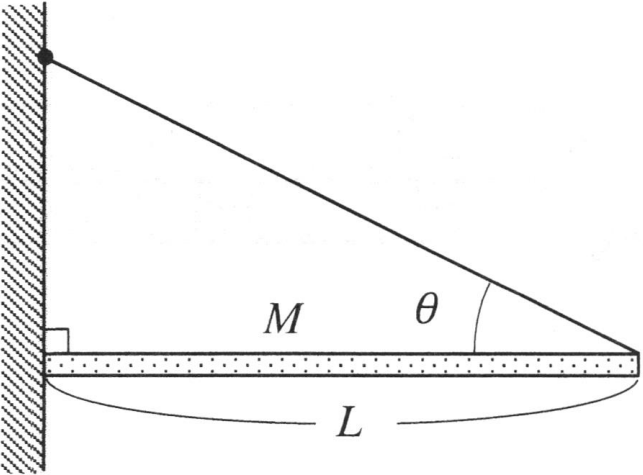
\includegraphics[width=\columnwidth]{../graphs/hamamatsu_23_2-1.png}
    \caption{}
  \end{minipage}
  \hspace{.1\columnwidth}
  \begin{minipage}[b]{.3\columnwidth}
    \centering
    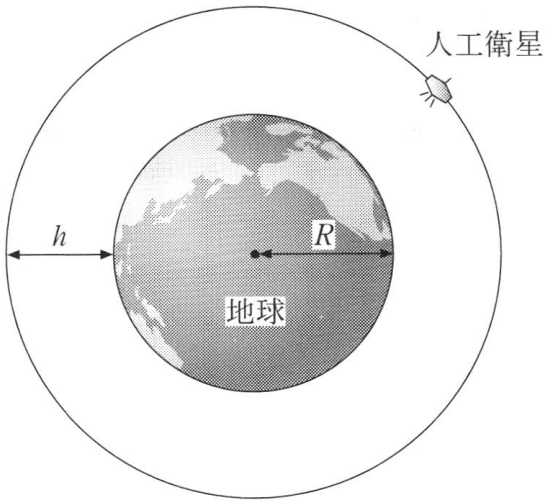
\includegraphics[width=\columnwidth]{../graphs/hamamatsu_23_2-2.png}
    \caption{}
  \end{minipage}
\end{figure}



% メモ
\begin{comment}

\end{comment}


%%%%%%%%%%%%%%%%%%

\clearpage

\qPart
%!TEX root = *.tex
%%%%%%%%%%%%%%%%%%
% カウンタのリセット
\setcounter{figure}{0}
% 問題文

以下の文章が正しい記述となるように,
\BrankNo{(3)},\BrankNo{(5)},\BrankNo{(6)},\BrankNo{(7)}の\{\quad\}内の選択肢のいずれかを選びなさい.
また,それ以外の\BrankNo{\ }には適切な語句あるいは式を記入しなさい.
式には文中に与えられた文字と,必要ならば,電気素量$e\unit{C}$を用いなさい.

物質は,電気をよく通す導体と,ほとんど通さない不導体(絶縁体)に大別される.
銅やアルミなどの金属は導体の,ガラスやプラスチックなどは絶縁体の代表例である.
また,電気の通しやすさが導体と絶縁体の中間の物質があり,これを\BrankNo{(1)}という.
導体である金属には,金属を構成している個々の原始に属さずに金属内を自由に動き回る電子があり,これを自由電子という.
金属に帯電体を近づけると自由電子が静電気力によって移動する.
そのため,帯電体が正に帯電している場合を考えると,
帯電体に近い側の表面には負の電荷が現れ,遠い側には正の電荷が現れる.
この現象を\BrankNo{(2)}という.
このとき,導体は\,\fbox{\quad (3)\quad\{帯電体側が高電位・帯電体が低電位・全体が等電位\}\quad}\,となる.
一方,絶縁体では,電子はすべて構成粒子(原子,分子,イオン)に属し,自由電子がないため,電気を通しにくい.
絶縁体の電子は構成粒子から離れないが,帯電体を近づけると,静電気力によって構成粒子に属している電子の位置がずれる.
これを\BrankNo{(4)}という.
ここで絶縁体をコンデンサーに挿入することを考えよう.
まず,2枚の金属板からなる平行板コンデンサーの一方の極板に正電荷を与え,
この正電荷と大きさの等しい負電荷をもう一方の極板に与える.
その極板間を絶縁体で満たすと,極板上の電荷がつくる電場は\,\fbox{\quad (5)\quad\{強め・弱め\}\quad}\,られる.
そのため,極板間の電位差は\,\fbox{\quad (6)\quad\{大きく・小さく\}\quad}\,なり,
コンデンサーの電気容量は\,\fbox{\quad (7)\quad\{大きく・小さく\}\quad}\,なる.

次に,金属導線に電池をつなぎ電流を流すことを考える.
電流の大きさは単位時間あたりに導線の断面を通過する電気量の大きさである.
金属導線内の自由電子は電場により加速されるが,
熱運動している陽イオンなどから抵抗力を受ける.
やがて電場による力と陽イオンなどからの抵抗力が釣り合い,
自由電子は一定の速さ$v\unit{m/s}$で電場と逆向きに移動するとして電流の大きさを求めてみよう.
導線の断面積は$A\unit{$\text{m}^2$}$,長さは$L\unit{m}$である.
導線の単位体積中の自由電子の数を\mbox{$N$\unit{個/$\text{m}^3$}}とすると,
電流の大きさは\BrankNo{(8)}\unit{A}となる.
導線の両端には電圧$V\unit{V}$が加えられており,導線内部に大きさ\BrankNo{(9)}\unit{V/m}の一様な電場が生じている.
自由電子はそれぞれ電場から大きさ\BrankNo{(10)}\unit{N}の静電気力を受けるため,
電子1個が単位時間あたり電場からされる仕事は\BrankNo{(11)}\unit{W}となる.
この仕事は電子にはたらいている抵抗力により熱的なエネルギーに変換される.
この熱を\BrankNo{(12)}という.
単位時間あたりに長さ$L$の導線から発生する熱量は\BrankNo{(13)}\unit{W}となる.
\BrankNo{(8)}の電流の大きさを$I$とすると,\BrankNo{(13)}の熱量を$I$と電圧$V$を用いて\BrankNo{(14)}\unit{W}と表すことができる.

次に,自由電子が陽イオンなどから受けている抵抗力の大きさは速さに比例すると考えよう.
その比例係数を$k$\unit{N$\cdot$s/m}とする($k>0$).
また,以下の(15),(16)の解答に$v$と$I$を用いてはならない.
抵抗力と電場による力が釣り合っているときの自由電子の速さは\BrankNo{(15)}\unit{m/s}である.
すべての自由電子がこの速さで運動していると考え,電流の大きさを\BrankNo{(8)}から求めると,この関係式はオームの法則を表している.この結果から導線の電気抵抗は\BrankNo{(16)}\unit{$\Omega$}と求められ,比例定数$k$に比例することがわかる.

\vspace{\baselineskip}

%\begin{comment}

\noindent
\textbf{【解答欄】}
\begingroup
\renewcommand{\arraystretch}{2}
\begin{table}[H]
  \centering
  \begin{tabular}{|p{.2\textwidth}|p{.2\textwidth}|p{.2\textwidth}|p{.2\textwidth}|}\hline
    (1)	& (2) & \multicolumn{2}{|l|}{(3)}\\\hline
    (4) &	(5)	& (6)	& (7) \\\hline
    (8)	& (9)	& (10) & (11) \\\hline
    \multicolumn{2}{|l|}{(12)} & (13) & (14) \\\hline
    \multicolumn{2}{|l|}{(15)} &	\multicolumn{2}{|l|}{(16)}\\\hline
  \end{tabular}
\end{table}
\endgroup

%\end{comment}

\begin{comment}
\noindent
\textbf{【解答】}
\begingroup
\renewcommand{\arraystretch}{2}
\begin{table}[H]
  \centering
  \begin{tabular}{|p{.2\textwidth}|p{.2\textwidth}|p{.2\textwidth}|p{.2\textwidth}|}\hline
    (1)	半導体& (2) 静電誘導& \multicolumn{2}{|l|}{(3) 全体が等電位}\\\hline
    (4) 誘電分極&	(5)	弱め& (6)	小さく& (7) 大きく\\\hline
    (8)	$eNAv$& (9)	$\dfrac{V}{L}$& (10) $\dfrac{eV}{L}$& (11) $\dfrac{evV}{L}$\\\hline
    \multicolumn{2}{|l|}{(12) ジュール熱} & (13) $eNAvV$& (14) $IV$\\\hline
    \multicolumn{2}{|l|}{(15) $\dfrac{eV}{kL}$} &	\multicolumn{2}{|l|}{(16) $\dfrac{k}{e^2n}\dfrac{L}{A}$}\\\hline
  \end{tabular}
\end{table}
\endgroup
\end{comment}



% メモ
\begin{comment}

\end{comment}


%%%%%%%%%%%%%%%%%%

\clearpage

\qPart
%!TEX root = *.tex
%%%%%%%%%%%%%%%%%%
% カウンタのリセット
\setcounter{figure}{0}
% 問題文

以下の\ajRoman{1}から\ajRoman{3}の文中にある\BrankNok{ア}から\BrankNok{シ}に適切な式や数値を入れよ.
ただし,必要ならば次の関係式を用いよ.
\begin{align*}
  \sin{A}+\sin{B} = 2\sin{\frac{A+B}{2}}\cos{\frac{A-B}{2}},\,
  \sin{A}-\sin{B} = 2\cos{\frac{A+B}{2}}\sin{\frac{A-B}{2}}
\end{align*}

\hang{\ajRoman{1}.}
放射能をもった一定量の原子核は,放射性崩壊により半減期$T$で時間とともに減少する.
\mbox{時間$t$}経過後に残っている原子核数$N$は,初期の原子核数を$N_0$とすると,$T$と$t$を用いて\BrankNok{ア}と表せる.
人工的に生成された原子番号53のヨウ素131の原子核は,$\beta$線を放出して崩壊($\beta$崩壊)し,16日後には初めの4分の1に減少するので,半減期$T$は\BrankNok{イ}日である.
このことから,48日後には,初めの\BrankNok{ウ}に減少すると推定できる.
なお,$\beta$崩壊したヨウ素131の原子核は,原子番号が\BrankNok{エ}のキセノン原子核となる.

\hang{\ajRoman{2}.}
X線は波長の短い電磁波で,真空中を光の速さ$c$と等しい速さで進む.
X線の波の性質を利用すると結晶の格子面間隔$d$を調べることができる.
いま,波長$\lambda$のX線を,格子面に対して角度$\theta$で入射する.
このとき,隣り合う格子面で反射されるX線の経路の長さに違いが生ずる.
そのため,隣り合う格子面で反射されたX線は,
波長$\lambda$,角度$\theta$および格子面間隔$d$の間に,
\nn を自然数として\BrankNok{オ}の条件が満たされるとき,
干渉して互いに強め合う.
このことから,波長$\lambda$が$0.154\,\text{nm}$のX線を用いて,$d$が$\BrankNok{カ}\,\text{nm}$以上の結晶の格子面間隔を調べることができる.\\
\hspace{.5zw}
一方,X線は粒子(光子)としての性質もある.
波長$\lambda$のX線光子は,真空中での運動量の大きさが\BrankNok{キ}で,
エネルギーの大きさが\BrankNok{ク}である粒子のようにふるまう.
ただし,プランク定数を$h$とした.

\hang{\ajRoman{3}.}
水面上に,三角形PRSの頂点P,R,Sの3点を考える.
いま,点Sと点Rを波源として,波長$\lambda$,振動数$f$,振幅$A$の波が減衰することなく,速さ$v$で広がっている.
点Pと点Sの間の距離は\x ,点Pと点Rの間の距離は\z で,
\x と\z は$\lambda$よりも十分に大きい($x \gg \lambda,\,z \gg \lambda$).
また,点Sと点Rの間の距離も$\lambda$より十分に大きい.
いま,時刻$t$で,点Sの波源による上下振動の変位が
$y_{\rm S}=A\sin{(\omega t+\frac{\pi}{3})}$,
点Rの波源による上下振動の変位が
$y_{\rm R}=A\sin{(\omega t+\frac{2\pi}{3})}$
と表せたとする.
ただし,$\omega =2\pi f$である.
このとき点Pには,時刻$t$で,点Sの波源から伝わる$y_1=\BrankNok{ケ}$の変位と,
点Rの波源から伝わる$y_2=\BrankNok{コ}$が現れる.
すなわち,点Pでは,点Sと点Rから伝わってきた波が重なる.
このとき点Pで観測される波の振幅は\BrankNok{サ}である.
このことから,点Pに現れる波の振幅は,波長$\lambda$,距離\x ,距離\z の間に,$m$を0以上の整数として,
\BrankNok{シ}の関係があるときに最大となる.


% メモ
\begin{comment}

\end{comment}


%%%%%%%%%%%%%%%%%%

\calcPage

\brankPage

\end{document}

